\section{Proceso} 

\begin{itemize}
	\item Cuadro de dialogo Navegador
	\begin{center}
	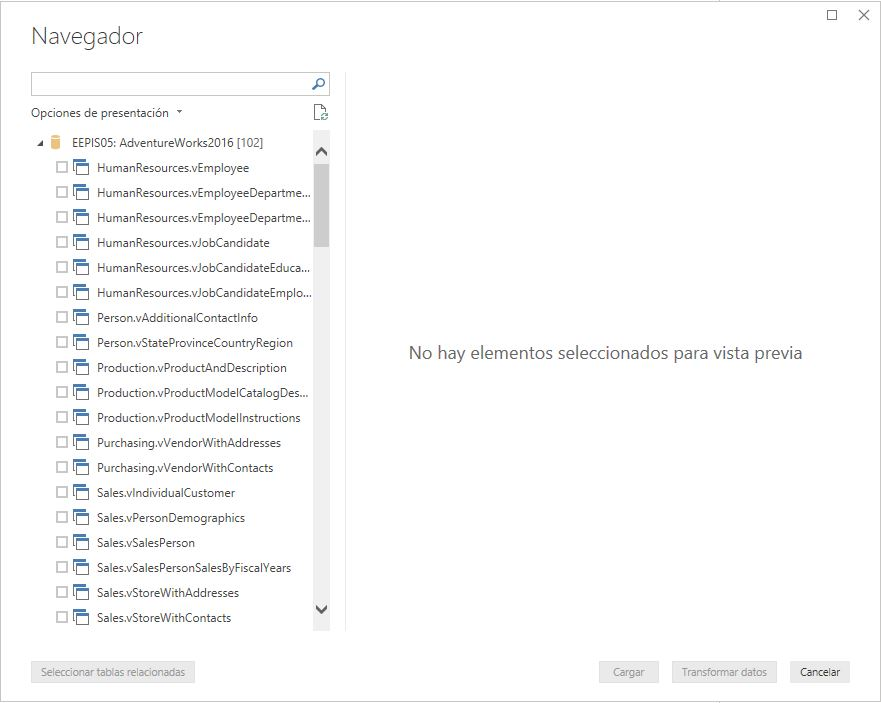
\includegraphics[width=10cm]{./Imagenes/Captura1} 
	\end{center}
\end{itemize} 

\begin{itemize}
	\item Seleccionando la vista Sales.vSalesPerson
	\begin{center}
	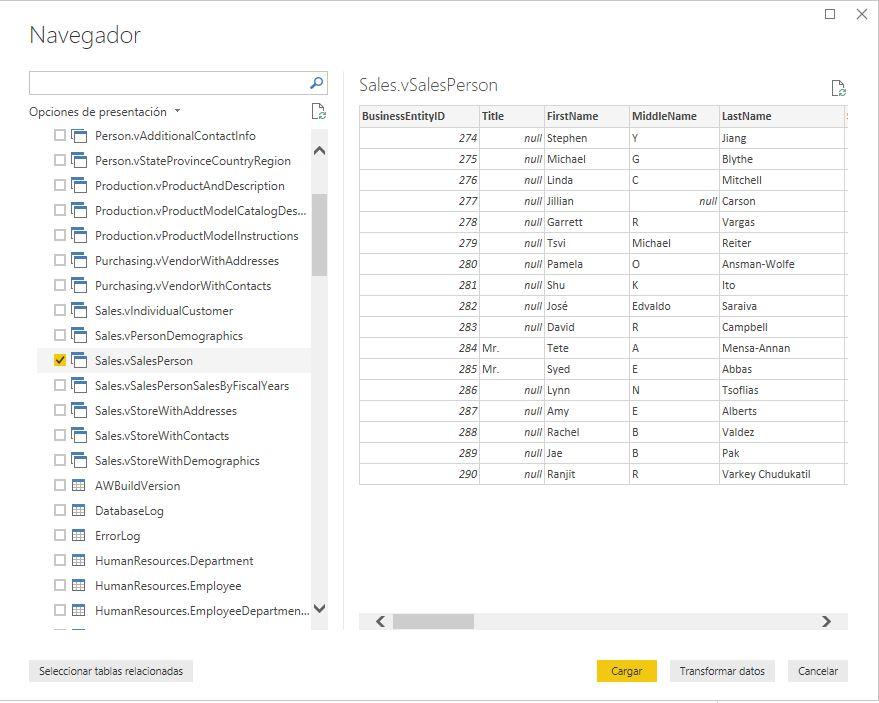
\includegraphics[width=10cm]{./Imagenes/Captura2} 
	\end{center}
\end{itemize} 

\begin{itemize}
	\item Seleccionando la vista Sales.vStoreWithDemographics
	\begin{center}
	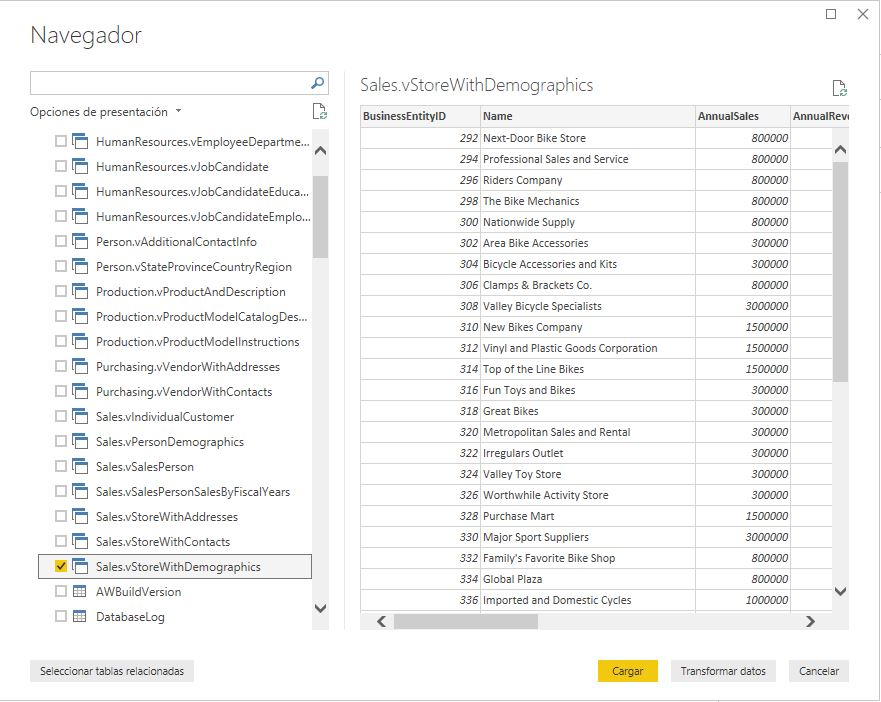
\includegraphics[width=10cm]{./Imagenes/Captura3} 
	\end{center}
\end{itemize} 

\begin{itemize}
	\item Opciones Avanzadas de obtener datos SQL Server, en la casilla sentencia SQL
	\begin{center}
	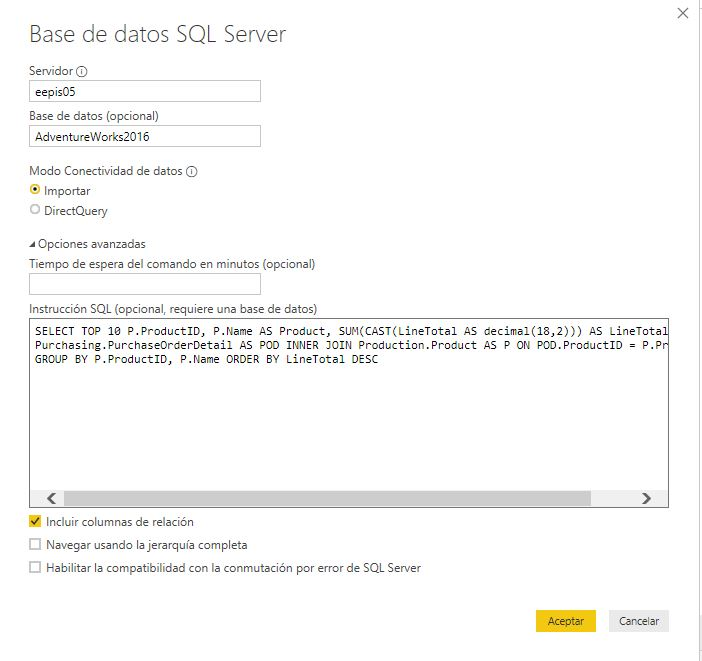
\includegraphics[width=10cm]{./Imagenes/Captura4} 
	\end{center}
\end{itemize} 

\begin{itemize}
	\item Panel Campos con las vistas seleccionadas
	\begin{center}
	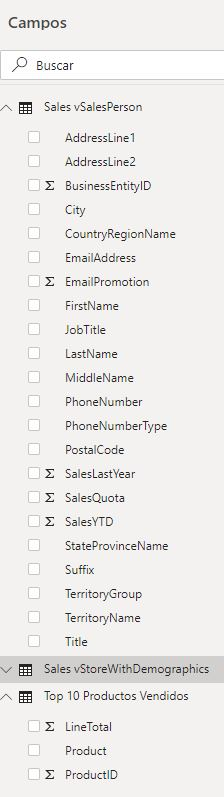
\includegraphics[width=5cm]{./Imagenes/Captura4-5} 
	\end{center}
\end{itemize} 

\begin{itemize}
	\item Reporte con Graficos Power Bi
	\begin{center}
	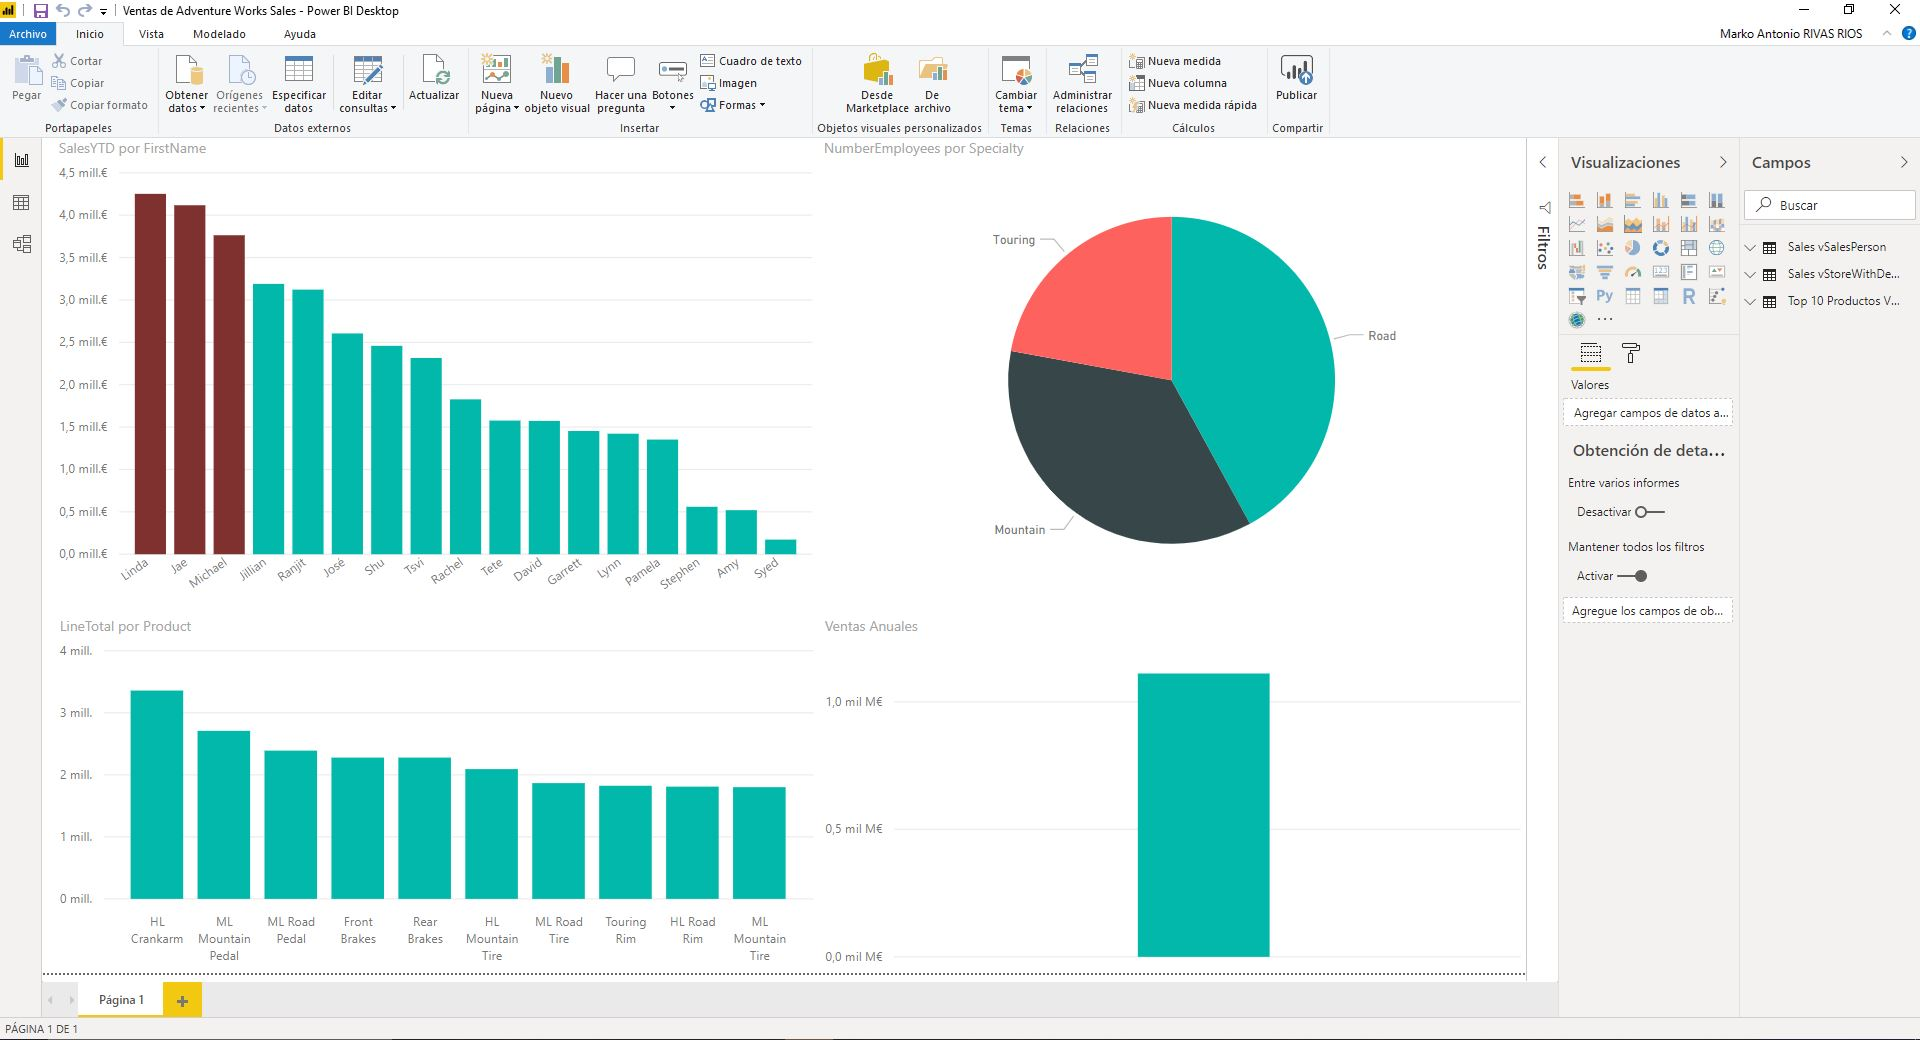
\includegraphics[width=13cm]{./Imagenes/Captura5} 
	\end{center}
\end{itemize} 

\begin{itemize}
	\item Reporte con Graficos portal de Power Bi 
	\begin{center}
	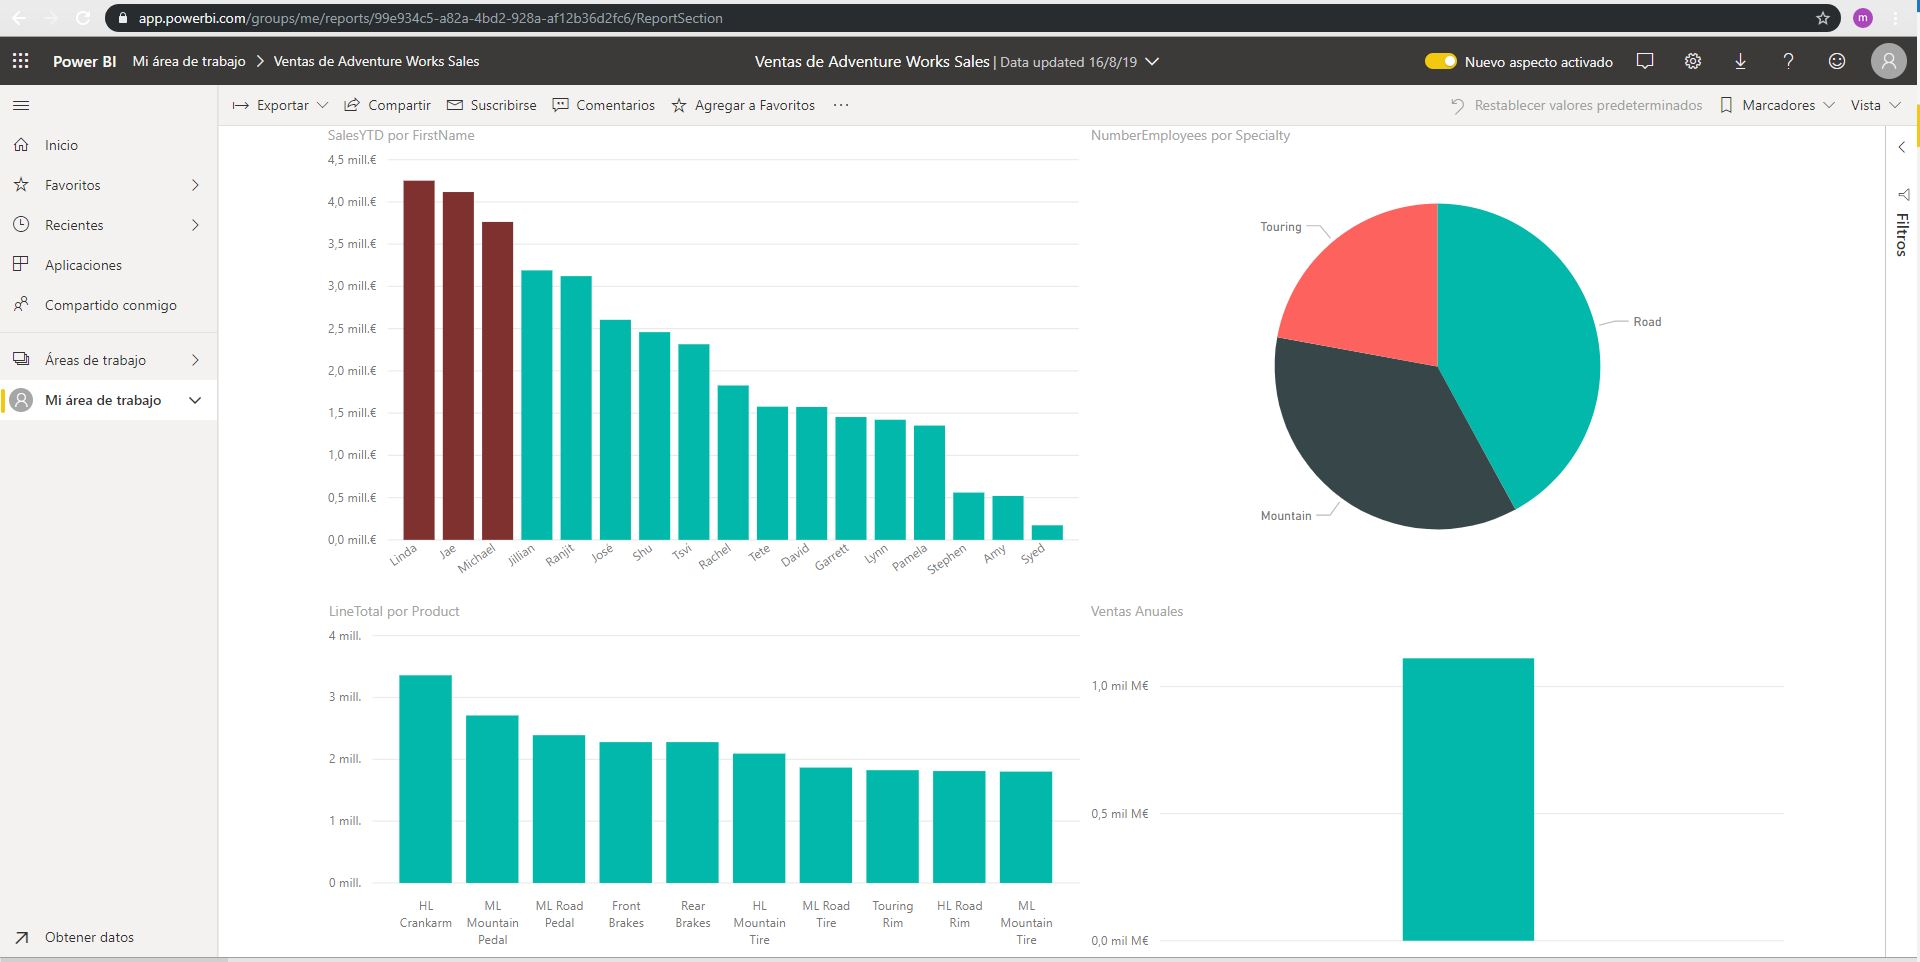
\includegraphics[width=13cm]{./Imagenes/Captura6} 
	\end{center}
\end{itemize} 
\begin{itemize}
	\item  Ruta del informe en el Portal de Power BI :
	\textbf{} \\
	https://app.powerbi.com/groups/me/reports/99e934c5-a82a-4bd2-928a-af12b36d2fc6/ReportSection
\end{itemize} 

